\documentclass{article}
\title{Atreus Keyboard Assembly}
\date{ }
\usepackage{graphicx}
\begin{document}
\setlength{\parindent}{0cm}
\maketitle
\section{Prerequisites}

In order to assemble your keyboard, you'll need your kit plus a few
other tools. The kit should contain these parts and a few spares:

\begin{itemize}
\item Case (top plate, switch plate, spacer, bottom plate)
\item Sandpaper
\item Finishing wax (mixture of beeswax and mineral oil)
\item Diodes (42)
\item Key switches (37 tactile or clicky, 5 red)
\item A-Star Micro controller
\item Machine screws and nuts (8 each, 16mm M3 size)
\item Key caps (40 normal, 2 long)
\item USB micro cable
\item Rubber feet
\end{itemize}

You'll also need to have these on hand:

\begin{itemize}
\item Soldering iron and solder
\item Wire cutters
\item Tape (masking tape works well)
\item Brush for applying finishing wax (a toothbrush will do)
\item Optional: ``helping hands'' stand
\end{itemize}

\vspace{1em}

The latest version of this document can always be found
online.\footnote{http://atreus.technomancy.us/assembly.pdf} If you're
reading a black-and-white printed copy, you may find some of the
photos clearer in color onscreen. This copy describes the
circuit-board-based kit. If you have an earlier hand-wired kit, see
the older assembly
guide.\footnote{http://atreus.technomancy.us/assembly-hand-wired.pdf}
The photos in this guide depict Cherry MX switches, but some kits ship
with Matias switches instead, which have a clear housing. The assembly
steps are the same in either case.

\section{Sanding}

Start by sanding down both sides of each piece. You may want to
hold two pieces together while sanding for strength or placing it on a
flat surface you don't mind scruffing up; too much pressure on a
single plate could damage it.

\vspace{1em}
\noindent\makebox[\textwidth]{%
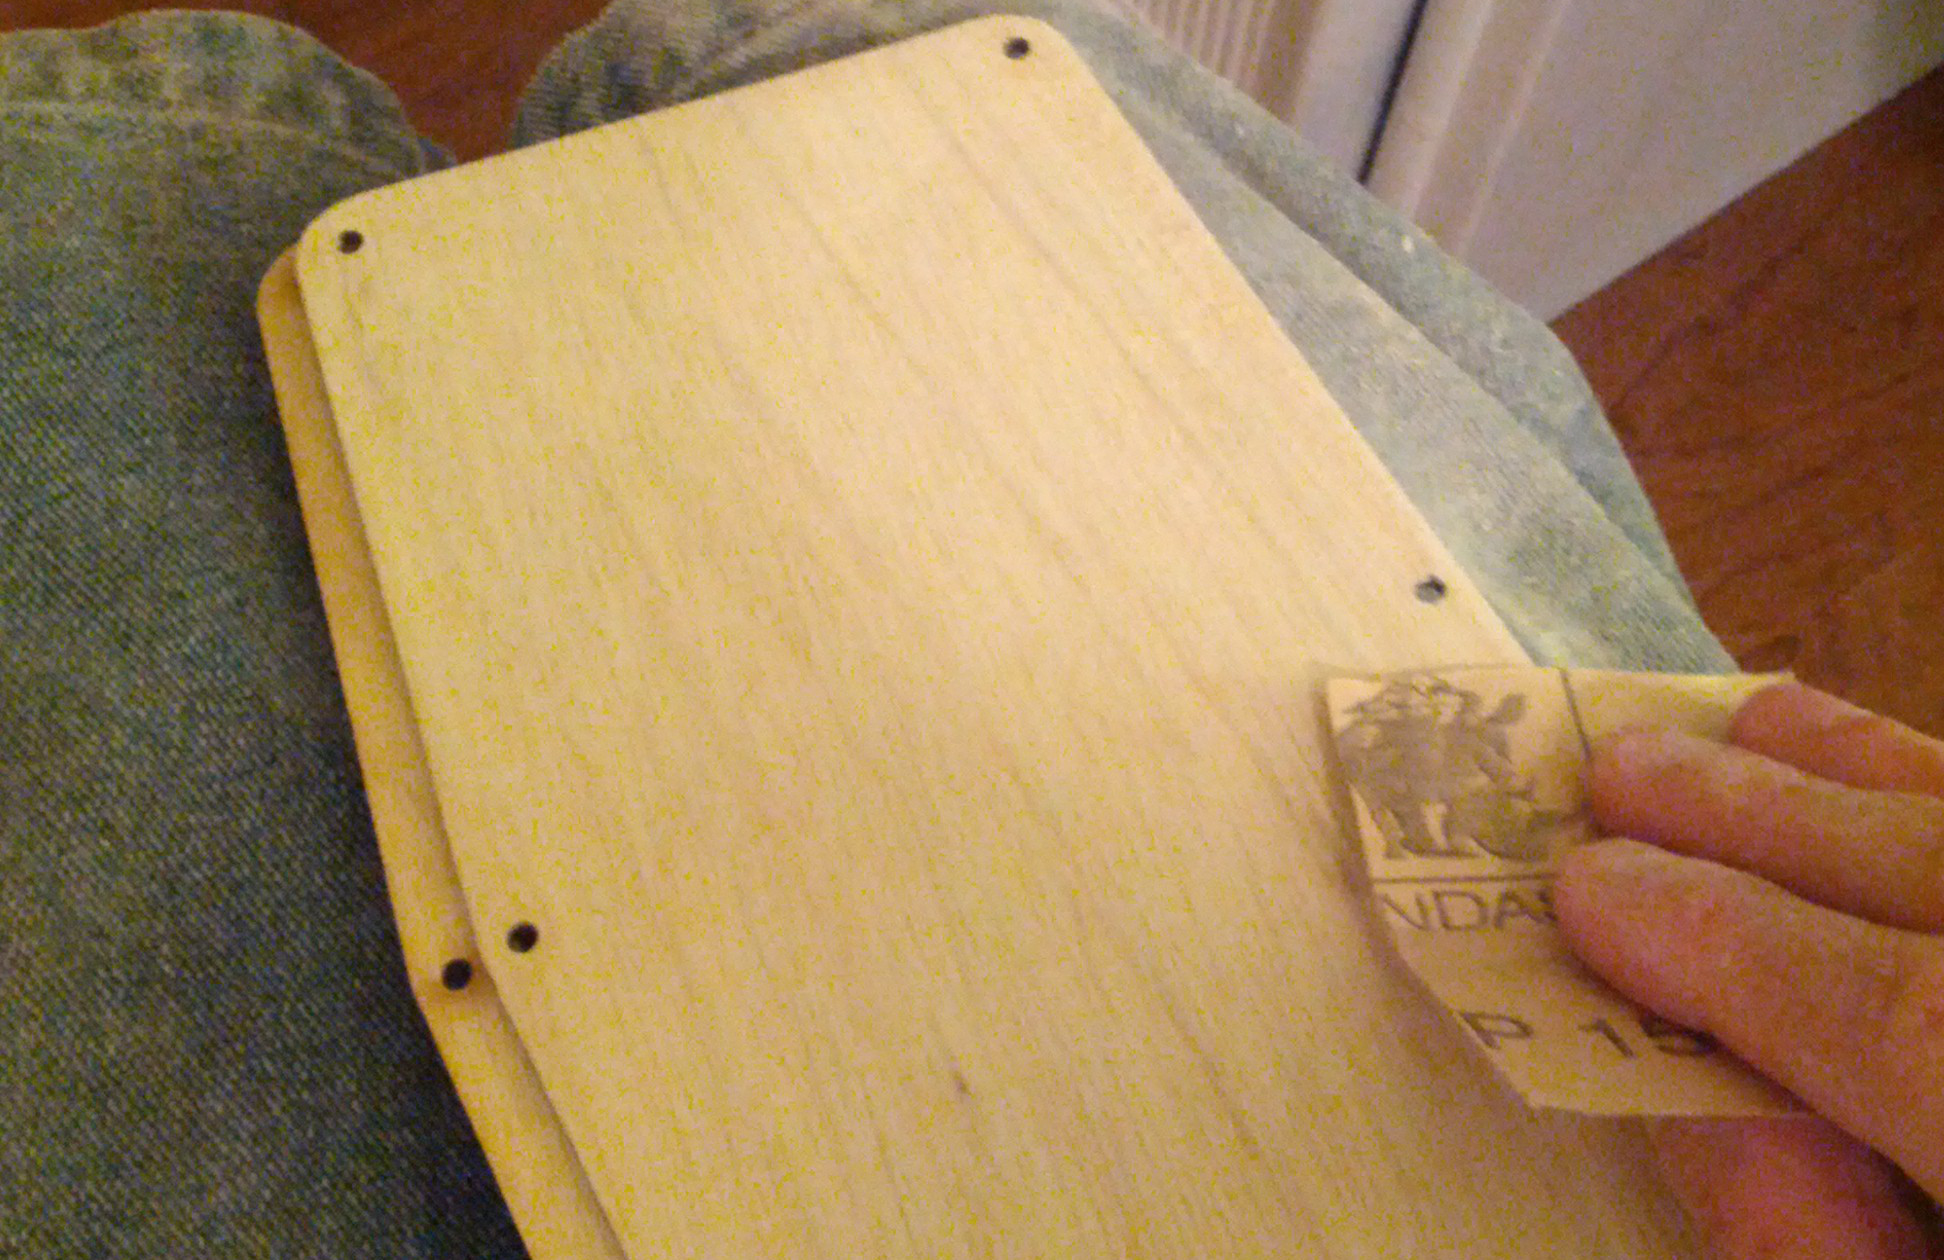
\includegraphics[width=\linewidth]{sanding.jpg}}
\vspace{1em}

Keep in mind that the top side of the top plate and the bottom side of
the bottom plate are the only surfaces that are exposed to the touch
once the keyboard is fully assembled, so these will need the most
attention when sanding. You can sand the other surfaces as well just
to get the scorch marks off, but you don't need to worry about how
smooth the inner surfaces feel to the touch. Be sure to get all the
wood dust off the pieces before you go on. A clean tack cloth or other
fine cloth works well.

\section{Finishing}

You have two options when it comes to finishing. The easiest way is to
proceed with the wax/oil mixture included in the kit. The other option
is to apply several layers of lacquer and wet sand it down in
between coats. This requires buying more supplies and takes significantly
longer, but it results in a shinier
finish.\footnote{http://atreus.technomancy.us/lacquer.gif} The steps
for the lacquered finish are described in a separate
document,\footnote{http://atreus.technomancy.us/lacquer.pdf} and the
rest of this section describes the quicker finishing method.

Open up the wax/oil mixture. Apply some to the brush and start
spreading it over one side of each case piece. The color of the wood
will darken as it absorbs the oil. Try to ensure it's spread
evenly. Be more generous with the oil on the outer exposed
surfaces. Once you've spread it with the brush, you can use your
fingers to work the wax into the wood more deeply.

\vspace{1em}
\noindent\makebox[\textwidth]{%
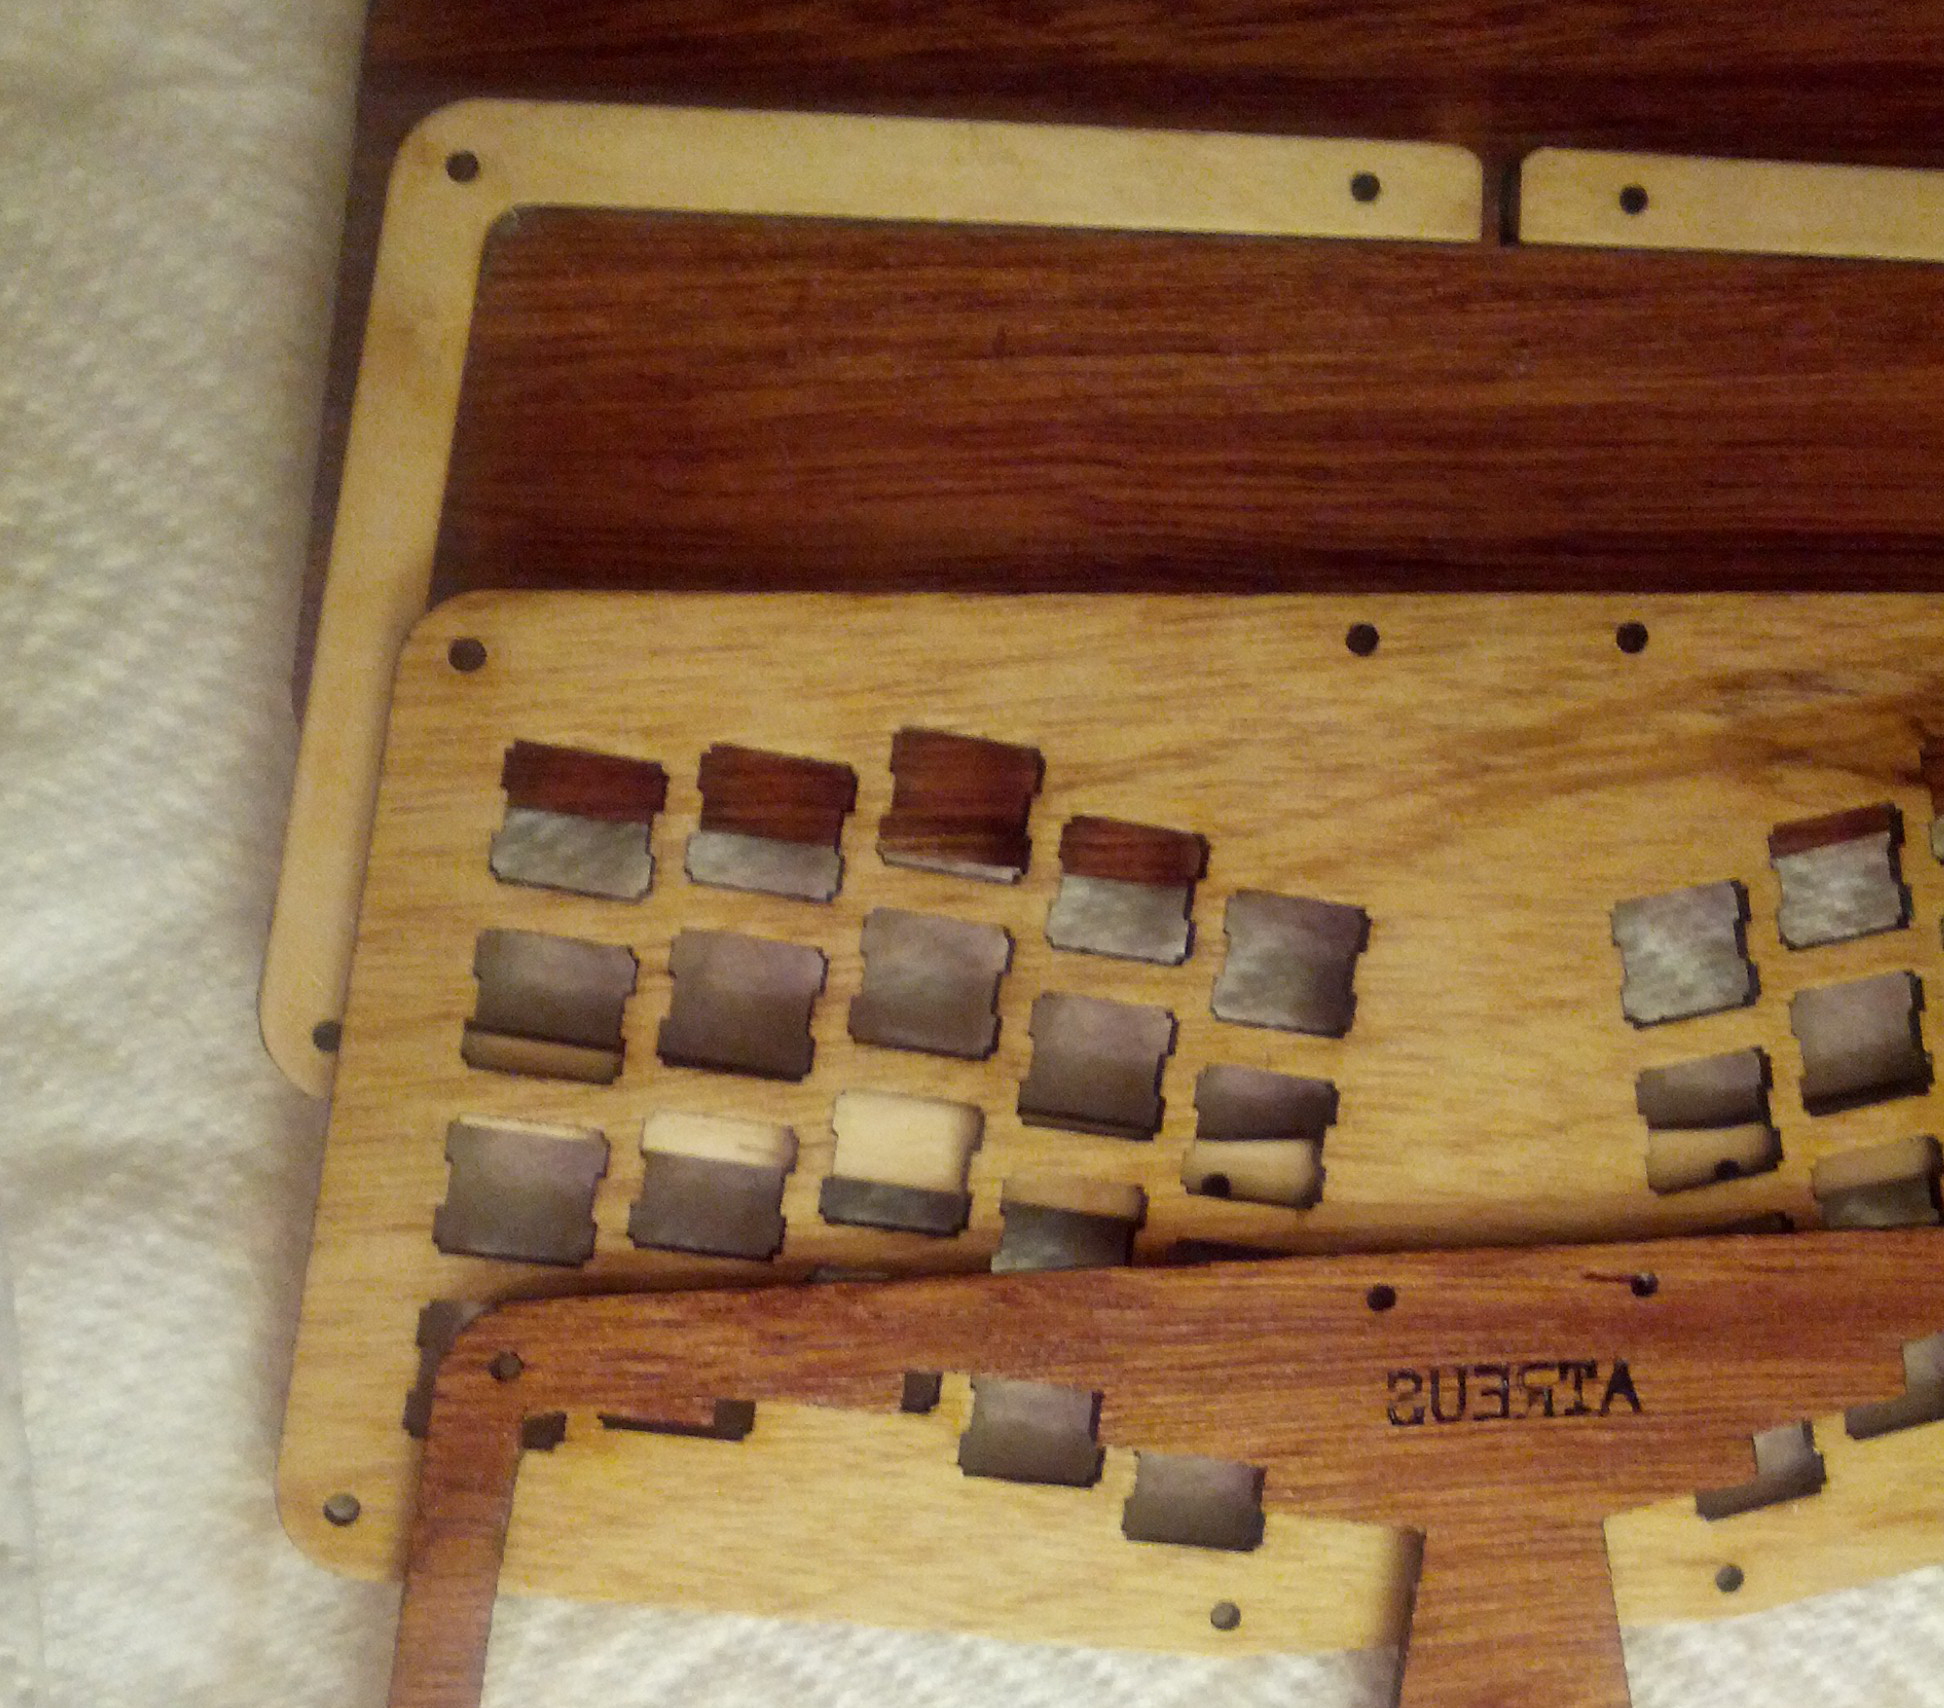
\includegraphics[width=\linewidth]{oiled.jpg}}
\vspace{1em}

As your brush goes over the edges of the laser-cut wood, it will get
dirty from charred wood particles. After you've finished oiling one
side of each piece, it's best to wash out the brush. Be sure it's
fully dry before going on.

\section{Drying Case}

Once one side of each piece is finished, you'll need to lay them out
for a half hour or so to let them dry. Once one side is dry, repeat
the process on the other side. After you've finished the construction
you can come back and add another few coats to the outermost surfaces
for a smoother texture. Once it's dried for a while, wipe the excess
off. While you're waiting, you can start soldering the diodes and
controller onto the circuit board, but don't solder any switches in
before the switch plate is ready or you'll just need to remove them
later.

\section{Diodes}

If you've never soldered before, there are plenty of good
introductions online.\footnote{This one from Adafruit is great:
  https://learn.adafruit.com/adafruit-guide-excellent-soldering/tools}
Coat the tip of the hot iron thinly with some solder before you
start. The key is to use the iron to heat both parts of the joint for
a second or two, then bring in a dab of the solder and let it melt and
stick to the component and the circuit board pad.

\vspace{1em}

Take five diodes at a time and bend them into a U shape. Place them
into the diode holes next to each switch slot on the reverse side of
the board. Each diode has a black band on it; the band should be
pointing in the direction of the arrow on the printed side of the
board. Once all five are in, bend the legs of the diodes outwards to
hold them in place, then flip the board over and solder them in place.

\vspace{1em}
\noindent\makebox[\textwidth]{%
  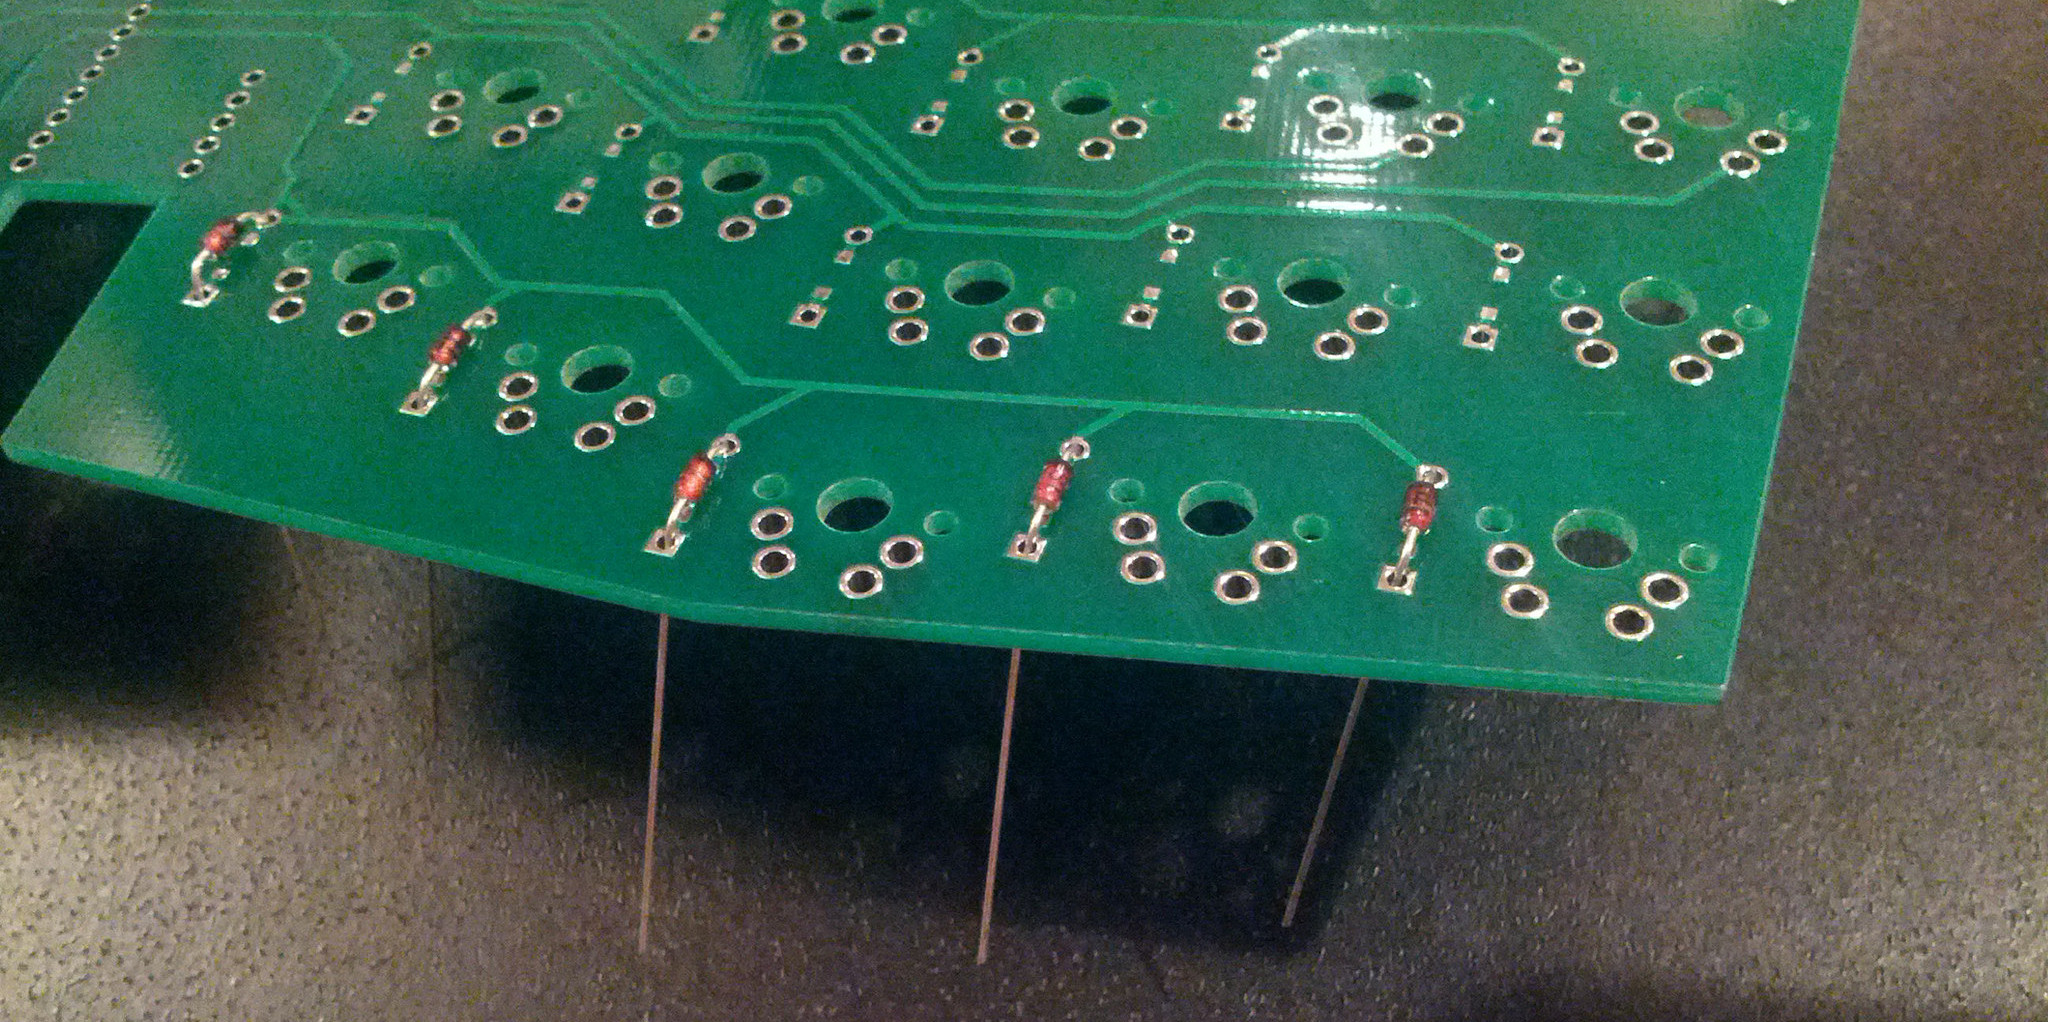
\includegraphics[width=\linewidth]{diodes.jpg}}
\vspace{1em}

In the photo the diodes are inserted from the back of the circuit
board, but it will work just as well to insert them from the front as
long as the black band is oriented correctly. Once they're soldered,
trim the diode legs with wire cutters. Grip the diode leg as you
trim it to keep it from flying across the room. Keep the diode legs;
they will be needed in the next step. Repeat until each diode position
is filled.

\section{Controller}

Once the diodes are in place, you can begin attaching the controller.
If the controller came in a pink bag with its own header pins, you may
be tempted to use them to connect the controller to the circuit
board. Don't do this--they are too big and will prevent the case from
closing when you're done.

\vspace{1em}

Take four trimmed diode legs and bend them into an L shape. Hold the
controller upside down and insert the diode legs into the holes at the
corners, (except for the VIN corner, which is not used; use the GND
hole instead as indicated in the picture below) fixing them in place
with tape. Try to get them to point straight.

\vspace{1em}
\noindent\makebox[\textwidth]{%
  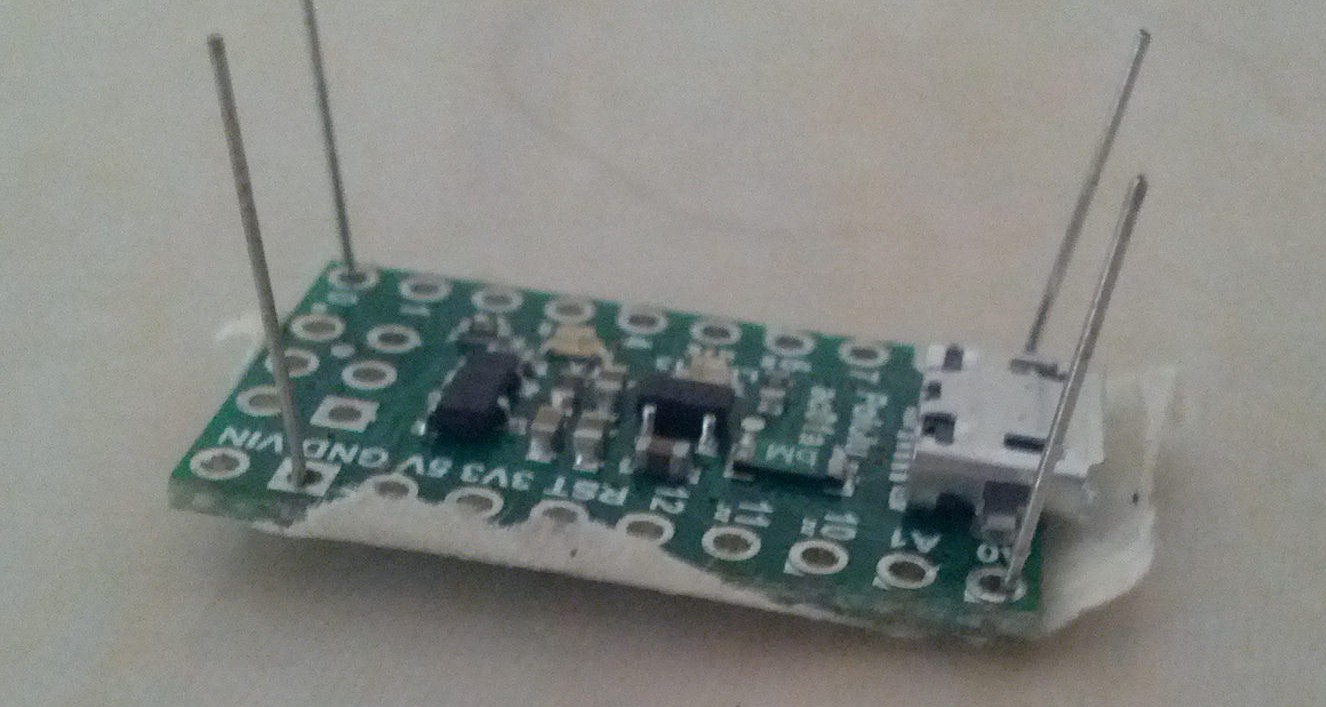
\includegraphics[width=\linewidth]{taped-pins.jpg}}
\vspace{1em}

Insert the legs into the circuit board. The port for the USB cable
should fit into the circuit board's notch in the middle. Solder the
diode legs into the circuit board and trim them. Then flip the whole
thing over, remove the tape, and solder them into the controller on
the other side, trying to ensure the controller is as close to the
board as possible.

\vspace{1em}
\noindent\makebox[\textwidth]{%
  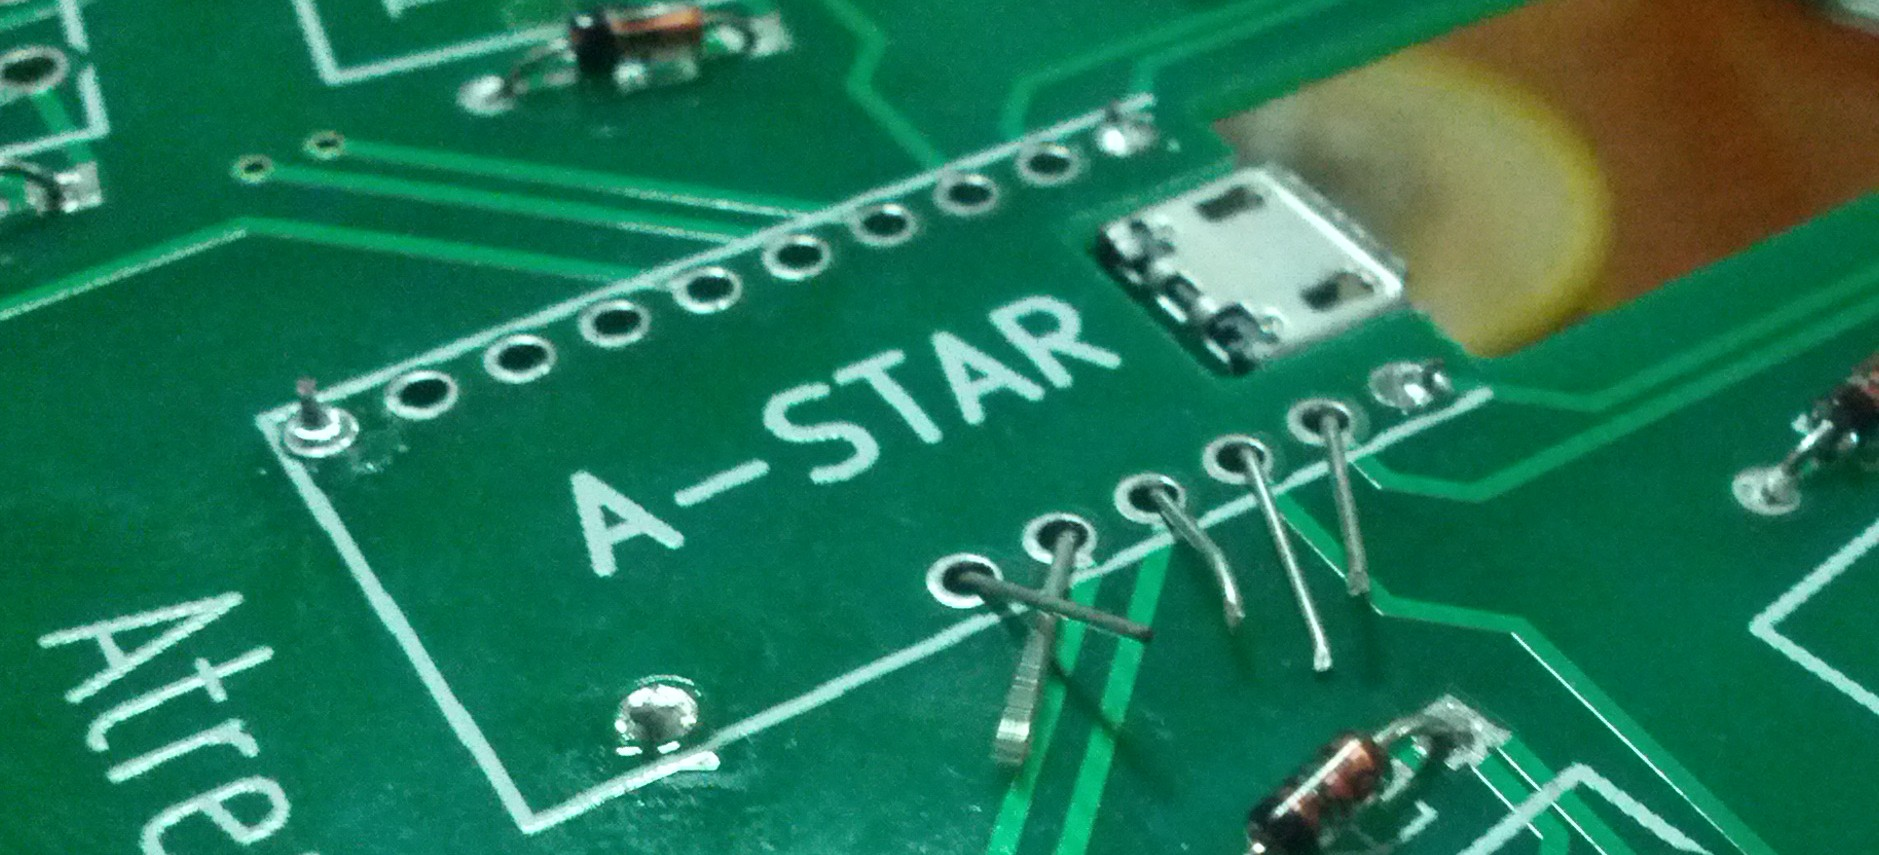
\includegraphics[width=\linewidth]{insert-pin.jpg}}
\vspace{1em}

Now that the controller is secured in place, bend some more diode legs
and put them in the other holes in the circuit board. You can do this
one side at a time. Use the same method of taping the bent ends in
place, flipping, and soldering the other side in place before going
back to solder the bent side. Trim as you go. Be sure to fill all the
``A-STAR'' holes in the circuit board.

\vspace{1em}

Before you go on, take the time to double-check the solder joints on
the controller. The solder should fill the hole completely without
spilling over to adjacent holes, and the legs should be secure. Also
check that all the diodes are facing the correct direction with the
black band pointing to the bottom of the board. Once the switches are
in place, the controller will be pinned between the switch plate and
the circuit board, making it difficult to make further changes to the
controller and its connections.

\section{Switches}

Next take four switches and place each switch in a corner of the
switch plate. (The case layer with all the holes in it.) The switches
should be oriented so that the side with pins is to the ``north'' of
the board so they fit into the holes in the circuit board. Put the
switch plate face-down on the table with the pins sticking
up. Carefully fit the circuit board over the protruding pins, trying
to get the pins to push as far through the circuit board as you can.
Solder those corners to hold the circuit board and the switch plate
together. The labeled side of the board should be face-up. Take care
that the switch pins are straight; pushing in a switch with a pin
that's a bit bent will bend it flat and prevent it from poking through
the circuit board.

\vspace{1em}

If your kit has five linear switches (non-tactile, usually red), you
can choose to use these for the modifiers or to leave the modifiers as
normal tactile keys. Since modifier keys are held down, they do not
benefit from tactility like normal keys do, so some people find they
prefer linear keys there, but this is a matter of personal taste.

\vspace{1em}

If you decide to use the linear switches, place them in the modifier
positions next and solder them in. These all go on the bottom row:
SW3:3, SW5:0, SW6:0, SW8:3, and SW9:3. Fill in the rest of the bottom
row with your primary switch type, and then fill in the leftmost
column as well. Note that the center two switches are oriented
sideways. The pins on them may need to be bent outwards a bit to get
them to fit into the circuit board.

\vspace{1em}
\noindent\makebox[\textwidth]{%
  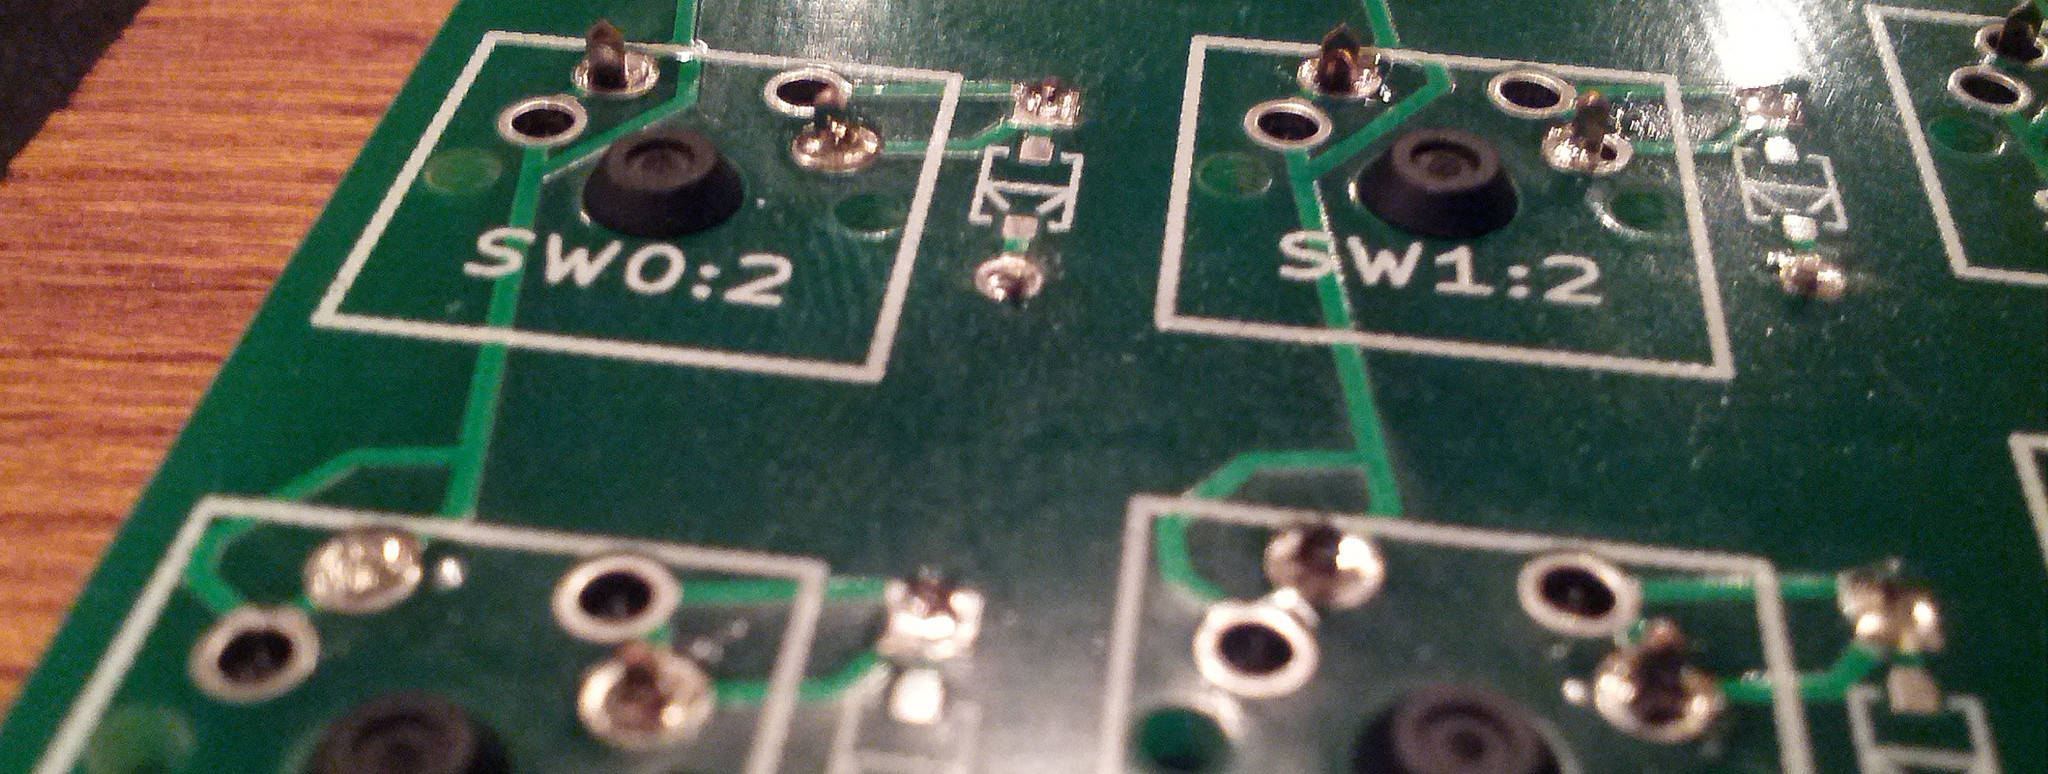
\includegraphics[width=\linewidth]{switches.jpg}}
\vspace{1em}

\section{Firmware}

With a full row and a full column installed you now have enough
switches installed to test every pin on the
microcontroller. Installing the firmware will allow you to spot
mistakes before the board is fully completed. Once all the switches
are in place it's a lot of work to go back and fix connections on the
microcontroller, but at this point it can be done by only removing a
handful of switches.

\vspace{1em}

Plug in the USB micro cable into the controller, and plug the other
side into your computer. Get a copy of the
firmware \footnote{Available at
  https://github.com/technomancy/atreus-firmware} and its
dependencies, \texttt{avrdude} and \texttt{gcc-avr}, linked in the
firmware readme\footnote{If you only want to use the default layout
  and don't want to bother with installing everything, the firmware
  readme also describes simpler steps for installing a pre-built
  firmware with the default layout}. The first time you upload the
firmware, you will have to use the backup reset to enter the
bootloader: take a diode leg or wire and touch one end to the reset
pin and one end to the ground pin. (These are the bottom-most two
exposed pins on the left-hand side of the controller when the keyboard
is facing down.) Touch them together twice in under a second and the
LED will begin pulsing in a different pattern from the original
blinking. This indicates it has entered the bootloader for 8 seconds.

\vspace{1em}

While in the bootloader, type \texttt{make upload USB=/path/to/usb}
from the firmware directory. The firmware should be
uploaded\footnote{See the firmware readme for instructions about
  determining the USB argument and customizing the layout.}, and it
should start acting as a keyboard. (At this point if you need to
upload it again, you can use the reset key instead of touching the
pins together.) Now would be a good time to test each switch that's
been placed so far.

\section{Wrapping Up}

If all the switches are registering key presses on your computer,
finish soldering the rest of the switches in.

\vspace{1em}

If there's a misbehaving switch, it's often caused by a cold
joint. Reflow the solder on both contacts of the switch and the diode
first; if that doesn't fix it, it may be the connection to the
controller. You can follow the traces for the columns back to the
middle, but the rows on the back of the board are obscured when the
keyboard is assembled. The bottom four pins on the left correspond to
the four rows, top to bottom.

\vspace{1em}

Re-melting the controller pin's solder for the affected row or column
is usually enough to get it working. First try the melting exposed
solder on the big circuit board; if that doesn't fix it you may need
to desolder some switches to get to the pins on the controller
itself. It's possible to remove switches using only your soldering
iron, but getting a desoldering pump is much more effective.

\vspace{1em}

If there is room between the head of the USB cable and the place where
the cable leaves the case, consider adding strain relief by wrapping
the cable with electrical tape at the point just below where it leaves
the case. This will make it so pulling on the cable does not dislodge
it from the controller.

\vspace{1em}

After the switches are all in and tested, close the case by placing
the switch plate on top of the spacer and bottom plate, placing the
top plate on it, and screwing it together with the nuts facing up. If the
controller was not attached close enough to the circuit board, it may
be necessary to sand down the USB connector in order to close the
case. Before you place the rubber feet on the bottom plate near the
corners, consider giving the outer case another coat or two of wax and
allowing it to dry. If the rubber feet don't stay on with the provided
adhesive, white glue may be needed to secure them.

\vspace{1em}

All that's left is to place the keycaps. The larger keycaps go on the
middle thumb keys.

\vspace{1em}

Congratulations. Enjoy your new keyboard. It will take a considerable
adjustment period to get used to it, but it should result in much more
comfortable and effective typing. Also remember that you're encouraged
to customize the layout to make it truly your own. Happy typing!

%% \noindent\makebox[\textwidth]{%
%% 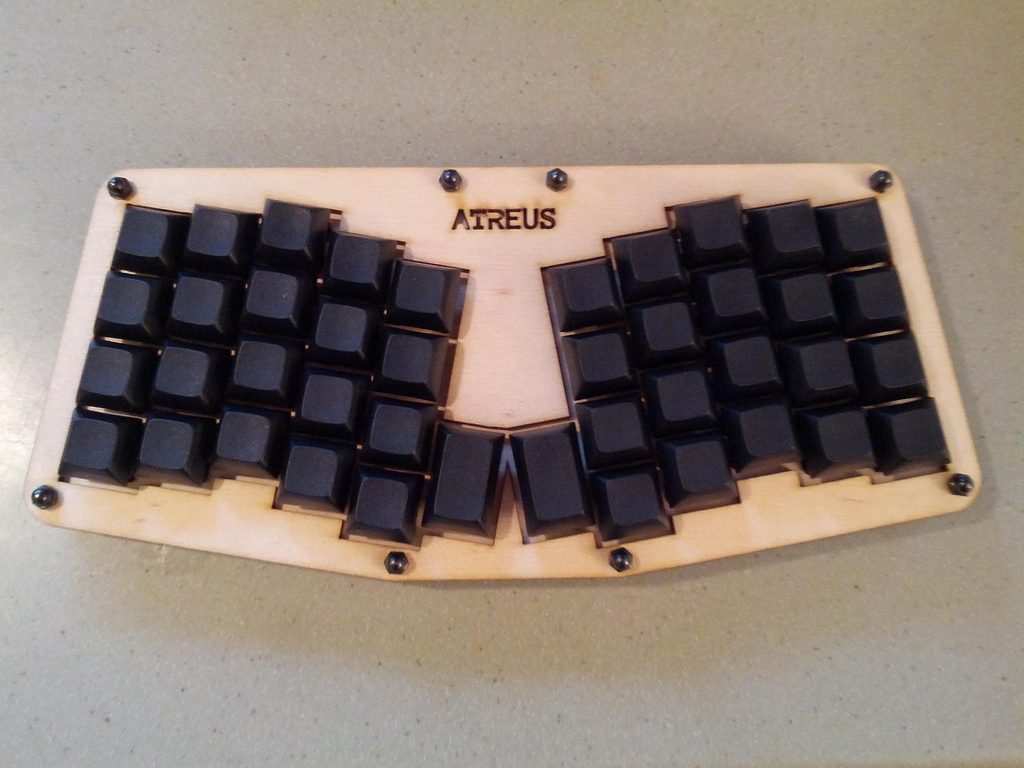
\includegraphics[width=\linewidth]{finished.jpg}}

\end{document}
